% 1. Set the top margin to 0.75 inch
\newcommand{\CLASSINPUTtoptextmargin}{0.75in}
% 2. Set the side margins to 0.75 inch
\newcommand{\CLASSINPUTinnersidemargin}{0.75in}
\newcommand{\CLASSINPUToutersidemargin}{0.75in}
\documentclass[conference,letterpaper]{IEEEtran}

% \documentclass[conference]{IEEEtran}
\IEEEoverridecommandlockouts
% The preceding line is only needed to identify funding in the first footnote. If that is unneeded, please comment it out.
\usepackage{cite}
\usepackage{amsmath,amssymb,amsfonts}
\usepackage{algorithmic}
\usepackage{graphicx}
\usepackage{textcomp}
\usepackage{xcolor}
\usepackage[hidelinks]{hyperref}
\usepackage{stfloats}
\usepackage{cuted}
\usepackage{caption}

\IEEEoverridecommandlockouts

% Tighten the wide-figure strip so the pipeline image sits close to the title.
\setlength{\stripsep}{2pt plus 1pt minus 1pt}

\def\BibTeX{{\rm B\kern-.05em{\sc i\kern-.025em b}\kern-.08em
    T\kern-.1667em\lower.7ex\hbox{E}\kern-.125emX}}

% 1.0 inch margin for first page
\renewcommand{\IEEEtitletopspaceextra}{0.25in}

\begin{document}

% \title{Risk-Aware Water-Surface Obstacle Detection and Warning via Segmentation and Depth Estimation}
\title{WARD: A Vision-Only Framework for Water-Surface Awareness and Risk Detection} %on Low-Cost ASVs}

\author{
    \IEEEauthorblockN{Yiran Zhou, Zheng Wang, Tianai Yan, Sacchin Sundar, Katherine A. Skinner}
    \IEEEauthorblockA{University of Michigan, Ann Arbor, USA \\
    \{yrzhou, zzww, tayanwu, sacchin, kskin\}@umich.edu}
}

\maketitle

% \begingroup
% \setlength{\abovecaptionskip}{24pt}
% \setlength{\belowcaptionskip}{8pt}
% \begin{strip}
%   \vspace{-2.5em}
%   \centering
%   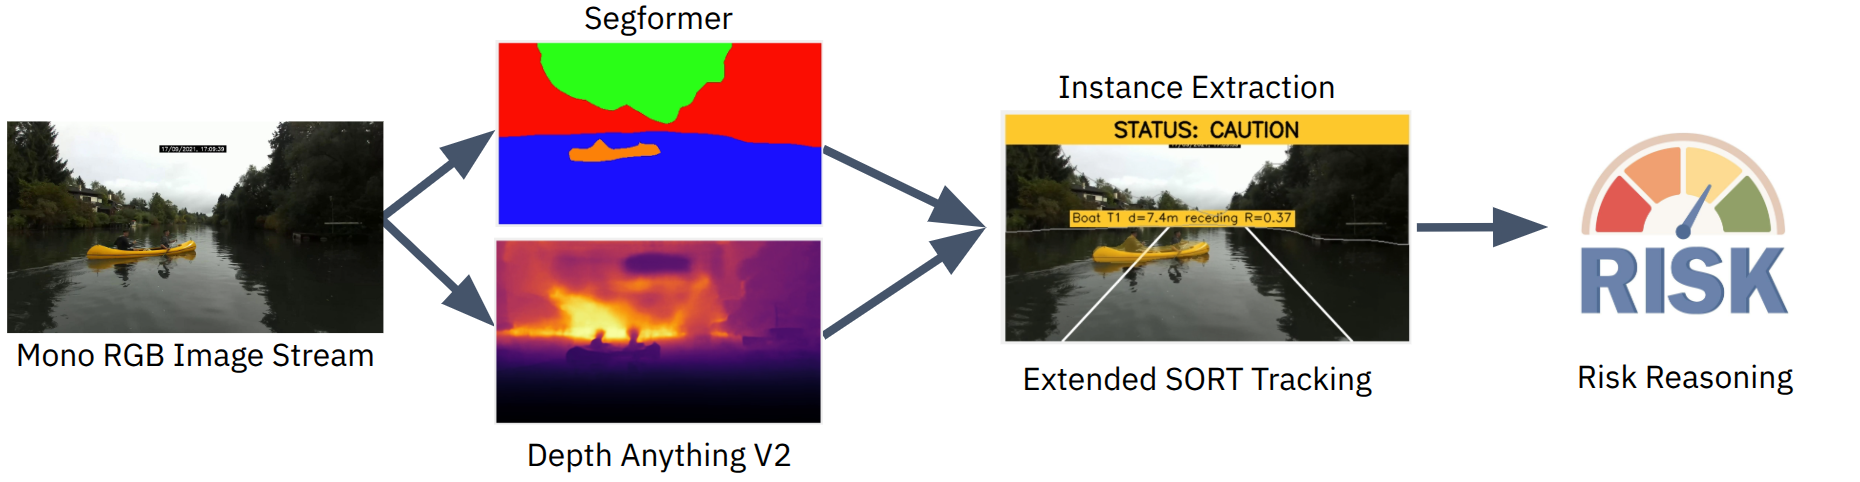
\includegraphics[width=0.9\textwidth]{images/pipeline.png}
%   \captionof{figure}{Overview of the proposed framework. Monocular RGB frames are processed by SegFormer and Depth Anything V2 to extract semantic and depth cues, which are then fused to generate actionable safety warnings.}
%   \label{fig:pipeline}
% \end{strip}
% \endgroup

\begingroup
\setlength{\abovecaptionskip}{6pt}
\setlength{\belowcaptionskip}{6pt}
\begin{strip}
  \vskip-2em
  \centering
  % 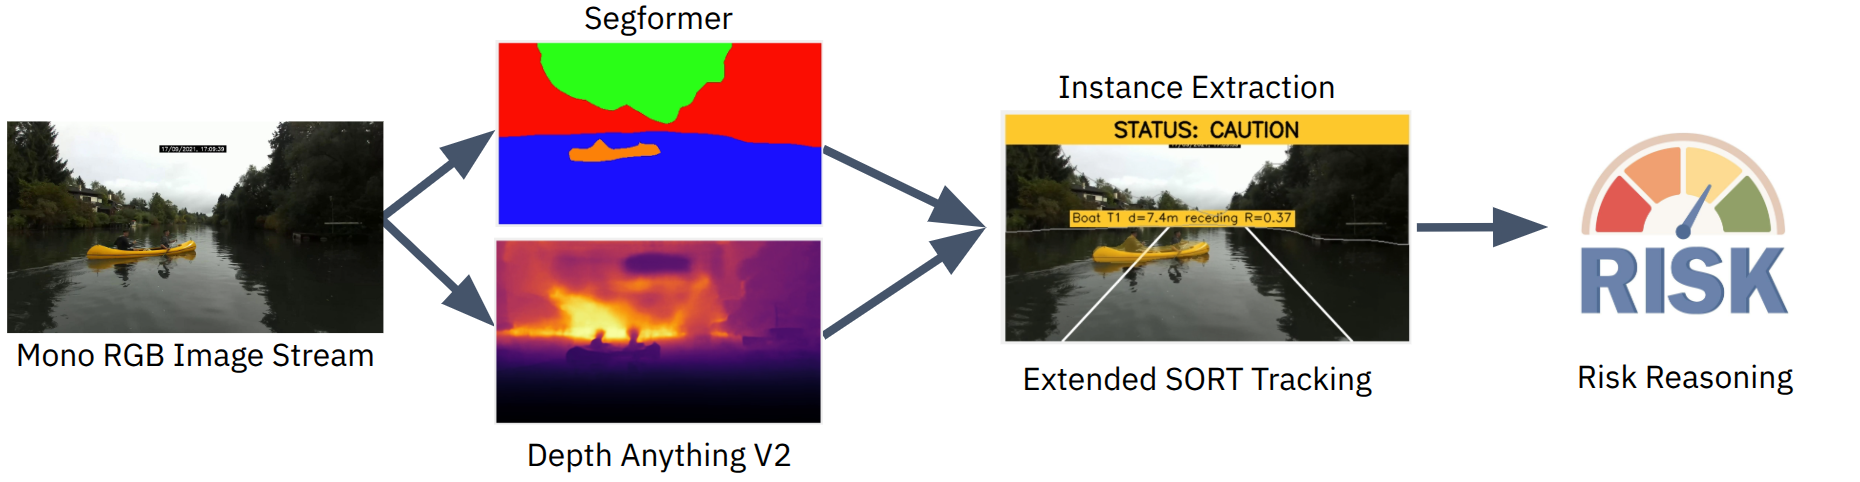
\includegraphics[width=0.9\textwidth]{images/pipeline.png}
  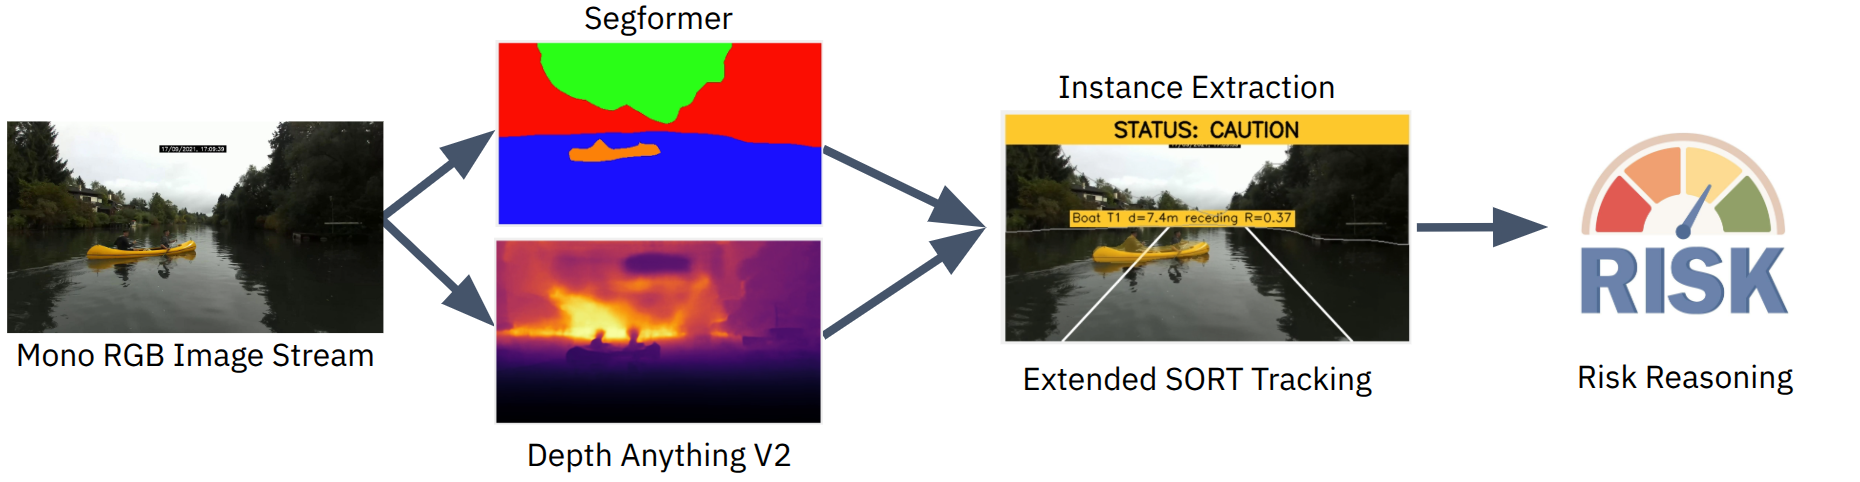
\includegraphics[width=\textwidth]{images/pipeline.png}
  \captionof{figure}{Overview of the proposed framework. Monocular RGB frames are processed by SegFormer and Depth Anything V2 to extract semantic and depth cues, which are then fused to generate actionable safety warnings.}
  \label{fig:pipeline}
\end{strip}
\endgroup

\begin{abstract}
Safe navigation for Autonomous Surface Vehicles (ASVs) requires both accurate obstacle detection and actionable risk assessment. We propose WARD (Water-surface Awareness and Risk Detection), a vision-only, risk-aware framework that can output safety assessments for low-cost ASVs. WARD fuses SegFormer semantic segmentation with radar-calibrated Depth Anything V2 monocular depth using a novel continuous collision-corridor risk model. The risk model reasons jointly about proximity, lateral offset, and semantic hazards to produce human-interpretable safety alerts. An extended SORT tracker ensures stable Time-to-Collision predictions by filtering monocular depth noise. Operating at 13.7 FPS on a consumer-grade GPU, WARD provides reliable, discrete safety warnings (SAFE, CAUTION, IMMEDIATE) for resource-constrained ASVs.
\end{abstract}

\section{Introduction}
Autonomous Surface Vehicles (ASVs) are increasingly deployed in unstructured maritime environments such as busy ports and marinas. These domains present unique perception challenges, including dynamic water reflections, waves, and low-profile hazards. %such as floating debris. 
While high-end platforms rely on active sensors like marine radar or LiDAR, small-scale ASVs demand low-cost, vision-only solutions that operate reliably under strict power and hardware constraints.

In safety-critical navigation, a gap exists between perception accuracy and operational safety: high accuracy in perception modules, such as object detection and segmentation, does not inherently translate into safe navigation. The fundamental question for an ASV is not whether an obstacle is perfectly segmented, but a more urgent one: \emph{``Does this obstacle pose an immediate collision risk?"} A vision system that returns raw detections without this risk-aware context can overwhelm the controller with data while failing to highlight the most pressing threats, such as treating a distant, harmless buoy and a swimmer in the immediate path as equally salient.

To bridge this gap, we propose WARD (Water-surface Awareness and Risk Detection), a vision-only (RGB), risk-aware framework that fuses SegFormer~\cite{xie2021segformersimpleefficientdesign} semantic segmentation with radar-calibrated Depth Anything V2~\cite{yang2024depthv2} monocular depth, as illustrated in Fig.~\ref{fig:pipeline}. WARD introduces a continuous collision-corridor risk model to reason jointly about proximity, lateral offset, closing velocity, and semantic hazard. By delivering actionable, real-time safety assessments (SAFE, CAUTION, and IMMEDIATE) from a single RGB stream, WARD offers a practical baseline for resource-constrained ASVs operating in dynamic environments.

% In summary, this paper contributes:
% \begin{itemize}
%     \item an end-to-end, vision-only pipeline that fuses semantic segmentation and monocular depth through connected-component instance extraction, avoiding specialized ranging hardware;
%     \item a radar-calibrated scaling strategy that restores near-range metric accuracy in a depth model pre-trained on road-driving imagery, within the band that matters most for collision warning;
%     \item a continuous collision-corridor risk score that unifies RSS-style geometric reasoning with semantic class weighting and closing-velocity amplification, in place of a binary safe/unsafe decision; and
%     \item a depth-augmented SORT tracker that jointly estimates bounding-box motion and closing velocity, yielding stable Time-to-Collision estimates despite noisy per-frame depth.
% \end{itemize}

%
% We evaluate WARD on real-world maritime sequences, prioritizing safety-oriented metrics over segmentation accuracy alone and ensuring that the system remains reliable and viable for real-time deployment on resource-constrained ASVs.
\section{Related Work}
% Our system draws on four lines of prior work: maritime semantic segmentation, monocular depth estimation, multi-object tracking, and collision-risk modeling.

\subsection{Maritime Semantic Segmentation}

Fully-convolutional architectures such as U-Net~\cite{ronneberger2015unetconvolutionalnetworksbiomedical} and the DeepLab family~\cite{chen2017rethinkingatrousconvolutionsemantic} established atrous convolution and spatial-pyramid pooling as standard tools for enlarging the effective receptive field, and transformer-based SegFormer~\cite{xie2021segformersimpleefficientdesign} later matched or exceeded these CNN baselines with a lighter hierarchical-attention design. In the maritime domain, WaSR~\cite{bovcon2021wasr} and MODD~\cite{Kristan2015} adapted this line of work to cope with wakes, reflections, and sun glitter, and the LaRS~\cite{zust2023larsdiversepanopticmaritime} and WaterScenes~\cite{yao2024waterscenesmultitask4dradarcamera} datasets have since consolidated training and evaluation data for ASV perception, with LaRS serving as our primary source. Nearly all of this work, however, optimizes pixel-level mIoU as the end goal, a metric that rewards precise boundaries but is silent on whether a hazard was detected at all. We instead treat segmentation as one stage of a downstream warning pipeline: evaluation is re-scaled around obstacle recall and inference latency, and SegFormer is extended with a boundary-prediction head, absent from the original design, to recover instance separation from a semantic-only backbone.

\subsection{Monocular Depth Estimation}

Monocular depth estimation has moved from dataset-specific regressors toward generalist foundation models. MiDaS~\cite{ranftl2020robustmonoculardepthestimation} showed that mixing depth datasets during training enables zero-shot relative-depth transfer, Depth Anything~\cite{yang2024depthanything} scaled this idea to tens of millions of unlabeled training images, and Depth Anything V2~\cite{yang2024depthv2} sharpened object boundaries with synthetic data and a larger teacher network. Diffusion-based methods such as Marigold~\cite{ke2025marigoldaffordableadaptationdiffusionbased} and DepthFM~\cite{gui2024depthfmfastmonoculardepth} trade inference speed for finer detail recovery. All of these models are trained primarily on road-driving and indoor imagery~\cite{gaidon2016virtualworldsproxymultiobject}; applied directly to open water, they show a consistent domain gap, with the horizon saturating and metric scale drifting away from physical units. Rather than retraining on scarce maritime depth data, we keep the pre-trained Depth Anything V2 representation intact and correct this drift with a single global scaling factor fit against radar ground truth, restoring near-range metric accuracy in the close-up range that matters most for collision warning.

\subsection{Multi-Object Tracking}

SORT~\cite{bewley2016simple} is a widely-used online tracker that combines a constant-velocity Kalman filter on 2D bounding boxes with Hungarian matching on IoU. DeepSORT~\cite{wojke2017simpleonlinerealtimetracking} augments SORT with a learned appearance embedding to reduce identity switches through occlusion. We adopt the SORT formulation for its low latency and minimal training requirements, but extend its 7-dimensional Kalman state to nine dimensions so that metric depth and its rate of change are tracked jointly with bounding-box dynamics.

\subsection{Collision-Risk Modeling}

Two lines of thought have shaped this area. The first is formal safety, exemplified by Mobileye's Responsibility-Sensitive Safety (RSS) framework~\cite{shalevshwartz2018formalmodelsafescalable}, which derives longitudinal and lateral safe distances from reaction time and braking capability, and by the ISO 22839 standard for forward collision mitigation~\cite{iso22839}. The second relies on domain-specific heuristics: the ship-domain concept of Fujii and Tanaka~\cite{fujii1971traffic} sizes a safe region around a vessel from its beam and operating speed, and recent ASV work adapts COLREGs rules to reactive collision avoidance~\cite{qu2022real}. Both typically collapse risk to a binary safe/unsafe decision and assume range measurements from active sensors. Our model keeps RSS's geometric decomposition into a forward-range term and a lateral-excess term, but replaces the kinematic safe-distance equations with a continuous exponential-decay score, weighted by obstacle class and modulated by closing velocity, so that approaching and receding obstacles at the same range are no longer treated as equally risky.

\section{Technical Approach}
% WARD's modular pipeline processes RGB frames through parallel SegFormer and Depth Anything V2 modules. 
% % These outputs are fused via our proposed continuous collision-corridor risk model to generate per-obstacle risk scores. To ensure temporal stability, these scores are smoothed by an extended SORT\cite{wojke2017simpleonlinerealtimetracking} tracker before being mapped to discrete warning levels.
% These outputs are fused via our continuous collision-corridor risk model to generate per-obstacle risk scores. To ensure stability, an extended SORT\cite{wojke2017simpleonlinerealtimetracking} tracker smooths these scores before mapping to discrete warning levels.

% \subsection{Segmentation and Calibrated Depth}
% We adopt SegFormer (MiT-B0) trained on the LaRS~\cite{zust2023larsdiversepanopticmaritime} dataset as our segmentation backbone. To enable instance separation from a semantic-only backbone, we extend it with a dual-head design: a 9-class semantic head and an auxiliary obstacle-boundary head, the latter used to split adjacent same-class instances during connected-component extraction. Depth is estimated using the Metric-Outdoor variant of Depth Anything V2, fine-tuned from the foundation model on synthetic Virtual KITTI data~\cite{gaidon2016virtualworldsproxymultiobject}. To correct scale bias from road-centric pre-training without retraining on scarce maritime data, we apply a single global scaling factor $s_{cal}=0.4$ calibrated once against radar ground truth from the WaterScenes dataset~\cite{yao2024waterscenesmultitask4dradarcamera} according to 
% $d_\mathrm{cal} = s_{cal} \cdot d_\mathrm{raw}$, 
% where $d_{\mathrm{raw}}$ is the raw output from the Depth Anything V2 model and $d_{\mathrm{cal}}$ represents the calibrated metric depth in meters. This adjustment restores near-metric accuracy in the critical $0$--$20$\,m close-up range, which is the primary zone for maritime collision warning. %For each segmented instance, a conservative depth is computed as the 5th percentile of its per-pixel depth distribution.

% \subsection{Risk Model and Extended Tracking}
% Based on the Responsibility-Sensitive Safety (RSS) framework~\cite{shalevshwartz2018formalmodelsafescalable}, we define a virtual forward collision corridor of width $W_\mathrm{boat} + 2M_\mathrm{lat}$ centered on the ASV heading, where $W_\mathrm{boat}$\ is the ASV beam width and $M_\mathrm{lat}$\ is the lateral safety margin. For an obstacle with forward distance $d_\mathrm{fwd}$ and lateral excess $e_\mathrm{lat}$ outside this corridor, we first compute a static risk baseline:
% \begin{equation}
%   R_\mathrm{base} = w_\mathrm{class} \cdot \exp\!\left(-d_\mathrm{fwd}/D_\mathrm{safe}\right) \cdot \exp\!\left(-e_\mathrm{lat}/L_\mathrm{safe}\right),
%   \label{eq:risk_base}
% \end{equation}
% where $w_\mathrm{class}$ is the semantic hazard weight, $D_\mathrm{safe}$\, is the forward decay constant, and $L_\mathrm{safe}$\, is the lateral decay constant. This baseline is amplified by a closing-velocity factor:
% \begin{equation}
%   R = R_\mathrm{base} \cdot \bigl(1 + \alpha_v \cdot \min(v_\mathrm{closing} / V_\mathrm{ref},\; 2)\bigr),
%   \label{eq:risk}
% \end{equation}
% where $v_\mathrm{closing}$ is the Kalman-filtered closing velocity, $V_\mathrm{ref}$\, is the reference speed, and $\alpha_v$ is the amplification factor. The continuous score $R$ is mapped to three discrete warning levels, SAFE ($R < 0.15$), CAUTION ($0.15 \le R < 0.50$), and IMMEDIATE($R \ge 0.50$), via threshold hysteresis with separate enter/exit values to suppress noise-induced flicker.
% To mitigate monocular depth noise, we extend the SORT tracker to a 9-D Kalman state $\mathbf{x} = [c_x, c_y, s, r, d, \dot{c}_x, \dot{c}_y, \dot{s}, \dot{d}]^\top$, where $(c_x, c_y)$, $s$, and $r$ denote the bounding-box center, scale (area), and aspect ratio; $d$ is the calibrated metric depth; and dotted variables represent their respective rates of change.
% The filter optimally balances depth observation noise against a constant-velocity process model. This yields smoothed estimates of the closing velocity, $v_{\mathrm{closing}} = -\dot{d} \cdot f_{\mathrm{fps}}$, and the Time-to-Collision, $TTC = d / v_{\mathrm{closing}}$, where $f_{\mathrm{fps}}$ is the system frame rate. These parameters feed directly into the risk model in Eq.~(\ref{eq:risk}) without requiring post-hoc exponential moving averages or windowing.

WARD's modular pipeline processes RGB frames through parallel SegFormer and Depth Anything V2 modules. These outputs are fused via our continuous collision-corridor risk model to generate per-obstacle risk scores. To ensure stability, an extended SORT tracker smooths these scores before mapping to discrete warning levels.

\subsection{Maritime Semantic Segmentation}
We adopt SegFormer (MiT-B0) trained on the LaRS~\cite{zust2023larsdiversepanopticmaritime} dataset as our segmentation backbone. To enable instance separation from a semantic-only backbone, we extend it with a dual-head design: a 9-class semantic head and an auxiliary obstacle-boundary head, the latter used to split adjacent same-class instances during connected-component extraction.

LaRS provides both semantic and instance-level annotations under conditions such as water reflections, sun glitter, and partially submerged obstacles. The MiT-B0 encoder was selected among the architectures we benchmarked for its accuracy--latency trade-off. The nine semantic classes, Static Obstacle, Water, Sky, Boat, Buoy, Swimmer, Animal, Float, and Other, are obtained by merging the LaRS panoptic categories. The two heads are trained jointly with a combined cross-entropy, Dice, and boundary binary cross-entropy loss, with class-specific weights (e.g., $5\times$ for Swimmer, $4\times$ for Buoy) to counter the severe class imbalance among hazard categories. At inference, the segmentation mask and calibrated depth map are fused: boundary pixels above a threshold $\tau_b=0.4$ are first suppressed to split adjacent same-class instances, and connected-component analysis is then applied to every non-background class (excluding Water and Sky) to isolate contiguous obstacle regions, discarding regions smaller than 300\,px as segmentation noise. Each surviving instance is assigned a representative depth equal to the 5th percentile of its pixel-wise depth distribution, a conservative estimate of its nearest point, and a normalized lateral offset $\ell \in [-1,1]$ relative to the image center.

\subsection{Monocular Depth Estimation}
Depth is estimated using the Metric-Outdoor variant of Depth Anything V2, fine-tuned from the foundation model on synthetic Virtual KITTI data~\cite{gaidon2016virtualworldsproxymultiobject}. To correct scale bias from road-centric pre-training without retraining on scarce maritime data, we apply a single global scaling factor $s_{cal}=0.4$ calibrated once against radar ground truth from the WaterScenes dataset~\cite{yao2024waterscenesmultitask4dradarcamera} according to 
$d_\mathrm{cal} = s_{cal} \cdot d_\mathrm{raw}$, 
where $d_{\mathrm{raw}}$ is the raw output from the Depth Anything V2 model and $d_{\mathrm{cal}}$ represents the calibrated metric depth in meters. This adjustment restores near-metric accuracy in the critical $0$--$20$\,m close-up range, which is the primary zone for maritime collision warning.

The scaling factor is fit using the sample subset of WaterScenes, which provides synchronized RGB and 4D-radar streams; radar points are projected onto image coordinates via the dataset's calibration to yield per-pixel metric ground truth. Even after calibration, accuracy degrades beyond 20\,m, and frame-to-frame estimates retain residual noise (median inter-frame variation of 0.28\,m on our evaluation sequences). Instead of pursuing tighter calibration, we design the downstream modules to tolerate this noise: the risk model relies on a conservative per-instance depth percentile rather than raw pixel depth, the tracker below smooths depth over time, and warning-level hysteresis absorbs the remaining flicker.

\subsection{Multi-Object Tracking}
To mitigate monocular depth noise, we extend the SORT tracker to a 9-D Kalman state $\mathbf{x} = [c_x, c_y, s, r, d, \dot{c}_x, \dot{c}_y, \dot{s}, \dot{d}]^\top$, where $(c_x, c_y)$, $s$, and $r$ denote the bounding-box center, scale (area), and aspect ratio; $d$ is the calibrated metric depth; and dotted variables represent their respective rates of change.
The filter optimally balances depth observation noise against a constant-velocity process model. This yields smoothed estimates of the closing velocity, $v_{\mathrm{closing}} = -\dot{d} \cdot f_{\mathrm{fps}}$, and the Time-to-Collision, $TTC = d / v_{\mathrm{closing}}$, where $f_{\mathrm{fps}}$ is the system frame rate. These parameters feed directly into the risk model in Eq.~(\ref{eq:risk}) without requiring post-hoc exponential moving averages or windowing.

Data association uses the Hungarian algorithm on an IoU cost matrix between predicted and observed boxes, with a minimum IoU of 0.20; unmatched detections spawn new tracks, tracks left unmatched for five consecutive frames are deleted, and a track is confirmed after two consecutive hits. Within that five-frame grace window, the filter continues to propagate depth and bounding-box motion forward under the constant-velocity model even without a matching detection, so a brief occlusion degrades the closing-velocity estimate gracefully rather than resetting it outright. The normalized lateral offset of each track is separately smoothed with an exponential moving average ($\alpha=0.4$), which keeps small shifts in the segmentation mask from producing abrupt changes in the lateral term of the risk model below.

\subsection{Collision-Risk Modeling}
Based on the Responsibility-Sensitive Safety (RSS) framework~\cite{shalevshwartz2018formalmodelsafescalable}, we define a virtual forward collision corridor of width $W_\mathrm{boat} + 2M_\mathrm{lat}$ centered on the ASV heading, where $W_\mathrm{boat}$\ is the ASV beam width and $M_\mathrm{lat}$\ is the lateral safety margin. For an obstacle with forward distance $d_\mathrm{fwd}$ and lateral excess $e_\mathrm{lat}$ outside this corridor, we first compute a static risk baseline:
\begin{equation}
  R_\mathrm{base} = w_\mathrm{class} \cdot \exp\!\left(-d_\mathrm{fwd}/D_\mathrm{safe}\right) \cdot \exp\!\left(-e_\mathrm{lat}/L_\mathrm{safe}\right),
  \label{eq:risk_base}
\end{equation}
where $w_\mathrm{class}$ is the semantic hazard weight, $D_\mathrm{safe}$\, is the forward decay constant, and $L_\mathrm{safe}$\, is the lateral decay constant. This baseline is amplified by a closing-velocity factor:
\begin{equation}
  R = R_\mathrm{base} \cdot \bigl(1 + \alpha_v \cdot \min(v_\mathrm{closing} / V_\mathrm{ref},\; 2)\bigr),
  \label{eq:risk}
\end{equation}
where $v_\mathrm{closing}$ is the Kalman-filtered closing velocity, $V_\mathrm{ref}$\, is the reference speed, and $\alpha_v$ is the amplification factor. The continuous score $R$ is mapped to three discrete warning levels, SAFE ($R < 0.15$), CAUTION ($0.15 \le R < 0.50$), and IMMEDIATE($R \ge 0.50$), via threshold hysteresis with separate enter/exit values to suppress noise-induced flicker.

Concretely, $W_\mathrm{boat}=2$\,m and $M_\mathrm{lat}=1$\,m, giving the lateral excess $e_\mathrm{lat} = \max(0,\ |d_\mathrm{lat}| - (W_\mathrm{boat}/2+M_\mathrm{lat}))$, where $d_\mathrm{lat} = \ell \cdot d_\mathrm{fwd} \cdot \tan(\theta_\mathrm{HFOV}/2)$. The decay constants are $D_\mathrm{safe}=12$\,m and $L_\mathrm{safe}=2$\,m; the per-class weight $w_\mathrm{class}$ runs from 1.0 for Boat down to 0.7 for Buoy and 0.3 for Static Obstacle; and the velocity term uses $V_\mathrm{ref}=3$\,m/s with $\alpha_v=1.0$. The multiplicative form requires both proximity and lateral alignment to be threatening at once, while the velocity term penalizes an approaching obstacle more heavily than a stationary or receding one at the same range. An obstacle directly ahead at $d_\mathrm{fwd}=0$ returns $R=w_\mathrm{class}$, and with the velocity factor included the score can reach $w_\mathrm{class} \cdot (1+2\alpha_v)$, so a high-weight obstacle closing rapidly can exceed 1.0 rather than saturate at a nominal ceiling. In practice, the enter/exit hysteresis thresholds for IMMEDIATE are set at 0.50 and 0.38, respectively, so a warning only drops once the score falls comfortably below the value that triggered it.

\section{Results}
% %\subsection{Perception Component Performance}
% We evaluated the segmentation backbone on the LaRS validation split. SegFormer achieves an obstacle recall of 96.51\%, substantially outperforming a DeepLab baseline (79.83\% recall) at comparable cost. This high recall is critical for safety-oriented ASV operation, where missed low-profile hazards such as buoys, swimmers, or floating debris can be catastrophic. For monocular depth, the evaluation was conducted using the radar data from the WaterScenes dataset, where the Base model provides a mean absolute error (MAE) of 4.04 m within the critical 0–20 m range. While the Large variant offers lower error (3.22\,m), its high latency is prohibitive for real-time edge navigation.

% %\subsection{End-to-End Pipeline and Efficiency}
% The integrated pipeline was evaluated on real-world maritime sequences from the MODD\cite{Kristan2015} dataset. As demonstrated by the qualitative results in Fig.~\ref{fig:pipeline_examples}, the system reliably distinguishes between stable and escalating risk states. The system maintains these transitions with high temporal stability; the warning distribution (62\% SAFE, 33\% CAUTION, 5\% IMMEDIATE) remained consistent with the obstacle dynamics, with no observed warning-level flicker.

% In terms of computational efficiency, the total system latency is 73.0 ms, sustaining approximately 13.7 FPS on a NVIDIA RTX 4060 GPU. Depth estimation is the primary bottleneck (38.7 ms), followed by segmentation (26.9 ms) and risk reasoning (7.4 ms). 
% % The system sustains 13.7 FPS (73.0 ms latency) on an RTX 4060 GPU. Latency is dominated by depth estimation (38.7 ms) and segmentation (26.9 ms), with minimal overhead for risk reasoning (7.4 ms).
% This low overhead for risk reasoning leaves significant headroom for future integration of higher-rate sensors or more complex fusion logic.

% \begin{figure}[t]
%     \centering
%     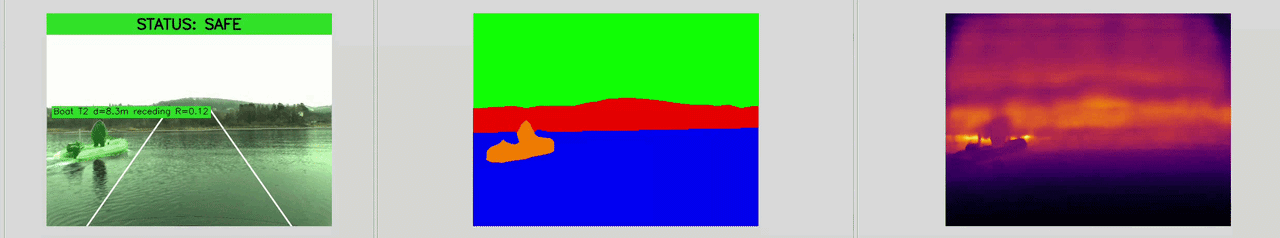
\includegraphics[width=\linewidth]{images/example1_safe.png}\\[2pt]
%     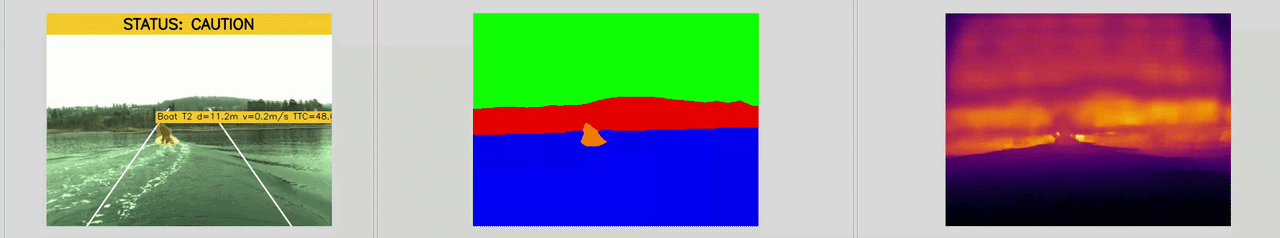
\includegraphics[width=\linewidth]{images/example1_caution.png}
%     \caption{Qualitative evaluation on a MODD sequence. As the tracked boat enters the virtual collision corridor, the system transitions from SAFE (top) to CAUTION (bottom). Each row shows the annotated RGB frame (left), semantic segmentation (center), and monocular depth map (right).\vspace{-4mm}}
%     \label{fig:pipeline_examples}
% \end{figure}

\subsection{Semantic Segmentation}
We evaluate the segmentation backbone against a DeepLab baseline on the LaRS~\cite{zust2023larsdiversepanopticmaritime} validation split, weighting obstacle recall and inference latency over aggregate pixel accuracy, in line with the safety-oriented evaluation stated in Section I. Table~\ref{tab:seg_compare} summarizes the comparison: SegFormer reaches 96.51\% obstacle recall, nearly 17 percentage points above DeepLab's 79.83\%, so far fewer hazardous obstacles go undetected. The gain comes at a latency cost: 29.74\,ms per frame against 15.44\,ms for DeepLab, though both remain compatible with real-time operation at typical ASV speeds.

\begin{table}[t]
\centering
\caption{Comparison of DeepLab and SegFormer on the LaRS validation set.}
\label{tab:seg_compare}
\begin{tabular}{lcc}
\hline
Metric & DeepLab & SegFormer \\
\hline
Obstacle Recall & 0.7983 & 0.9651 \\
Obstacle Precision & 0.9648 & 0.9737 \\
Avg.\ Latency (ms) & 15.44 & 29.74 \\
\hline
\end{tabular}
\end{table}

Per-class IoU on a held-out set of 198 test images (Table~\ref{tab:per_class_iou}) shows where this recall advantage comes from and where the model still struggles. Dominant background classes are segmented almost perfectly, 0.9703 for Water and 0.9618 for Sky, and large static obstacles reach 0.9056. Small or infrequent hazard classes fare far worse: Buoy scores 0.2036, Swimmer 0.4254, and Animal (0.0068) and Float (0.0000) are essentially unrecovered, pulling the class-averaged mIoU down to 0.4823 despite the strong recall figure above. The gap reflects severe class imbalance in LaRS together with the small spatial footprint and appearance variability of these objects, and it matters less for our purposes than it would elsewhere, since the downstream risk model depends on obstacle presence and a conservative depth percentile rather than a pixel-accurate boundary.

\begin{table}[t]
\centering
\caption{Per-class IoU on the segmentation test set (SegFormer).}
\label{tab:per_class_iou}
\begin{tabular}{lc}
\hline
Class & IoU \\
\hline
Static Obstacle & 0.9056 \\
Water & 0.9703 \\
Sky & 0.9618 \\
Boat & 0.6230 \\
Buoy & 0.2036 \\
Swimmer & 0.4254 \\
Animal & 0.0068 \\
Float & 0.0000 \\
Other & 0.2442 \\
\hline
mIoU & 0.4823 \\
\hline
\end{tabular}
\end{table}

Figure~\ref{fig:seg_qual} contrasts DeepLab and SegFormer predictions on a representative frame. Both recover the dominant sky and water regions, but DeepLab fragments the thin obstacle band near the waterline, while SegFormer preserves a more continuous region that matches the ground-truth overlay more closely, consistent with its higher measured recall.

\begin{figure*}[t]
\centering
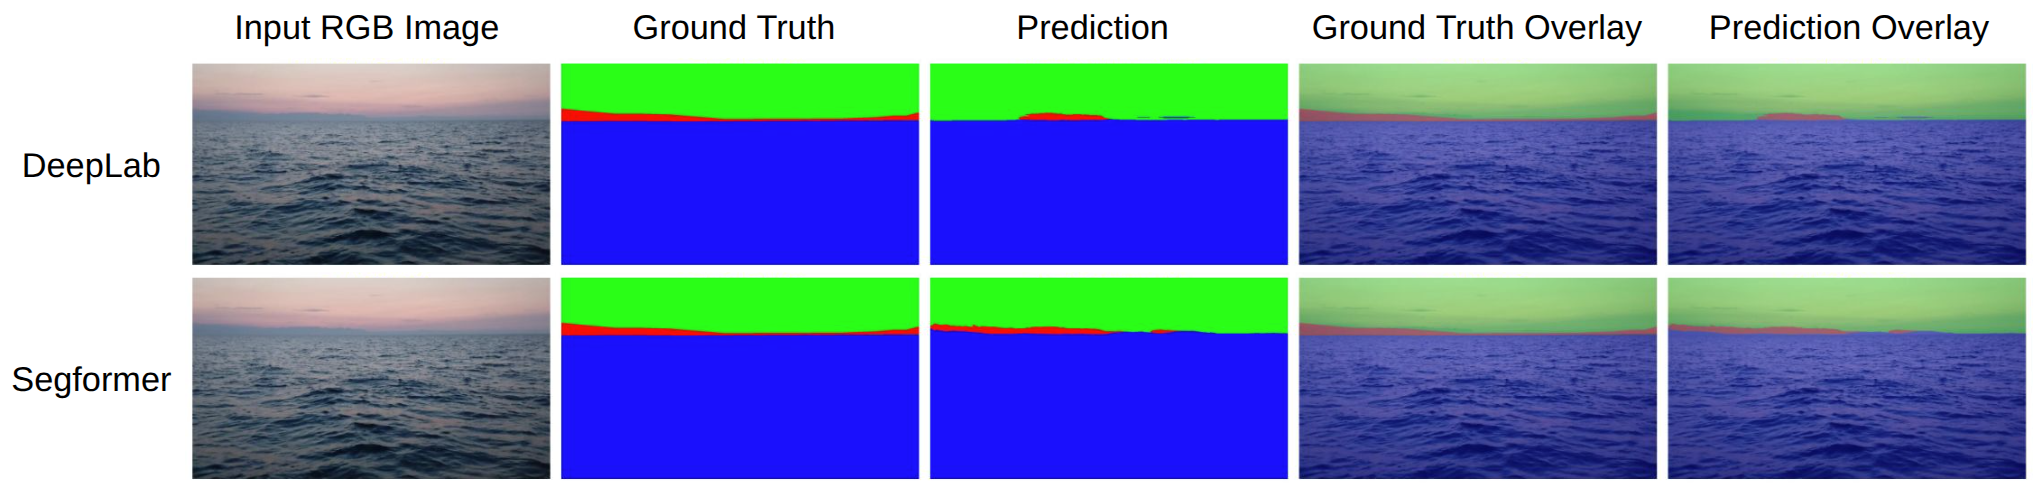
\includegraphics[width=\textwidth]{images/deeplabVSsegformer.png}
\caption{Qualitative comparison of DeepLab and SegFormer on a representative maritime frame.}
\label{fig:seg_qual}
\end{figure*}

\subsection{Monocular Depth Estimation}
We benchmark three variants of the Metric-Outdoor Depth Anything V2 model, small, base, and large, against 33,648 radar-aligned points drawn from the WaterScenes~\cite{yao2024waterscenesmultitask4dradarcamera} sample subset, applying the calibration described in Section III-B. Table~\ref{tab:depth_compare} reports accuracy within the 0--20\,m range that matters most for collision warning. The large model is the most accurate, MAE 3.215\,m with an Est/GT ratio of 1.008 (near-metric scale), but also the slowest at 0.710\,s per image; the small model is fastest (0.149\,s) but least accurate (MAE 4.434\,m). We deploy the base variant in the pipeline as a middle ground (MAE 4.039\,m at 0.279\,s per image): the large model's latency is incompatible with real-time navigation, and the small model's error is too high for reliable collision warning.

\begin{table}[t]
\centering
\caption{Depth model comparison within 0--20\,m.}
\label{tab:depth_compare}
\begin{tabular}{lccc}
\hline
Model & MAE (m) & RMSE (m) & Est/GT \\
\hline
Small & 4.434 & 5.719 & 0.787 \\
Base & 4.039 & 5.363 & 0.887 \\
Large & 3.215 & 4.471 & 1.008 \\
\hline
\end{tabular}
\end{table}

Even after calibration, accuracy degrades beyond 20\,m: median inter-frame depth variation is 0.28\,m on our evaluation sequences, and predictions saturate near the model's built-in depth ceiling of approximately 80\,m, which the calibration factor $s_{cal}=0.4$ maps down to roughly 32\,m. Figure~\ref{fig:depth_qual} shows this behavior directly: the estimated-versus-ground-truth scatter clusters tightly along the diagonal at short range but drifts and flattens as distance grows toward the saturation point.

\begin{figure}[t]
\centering
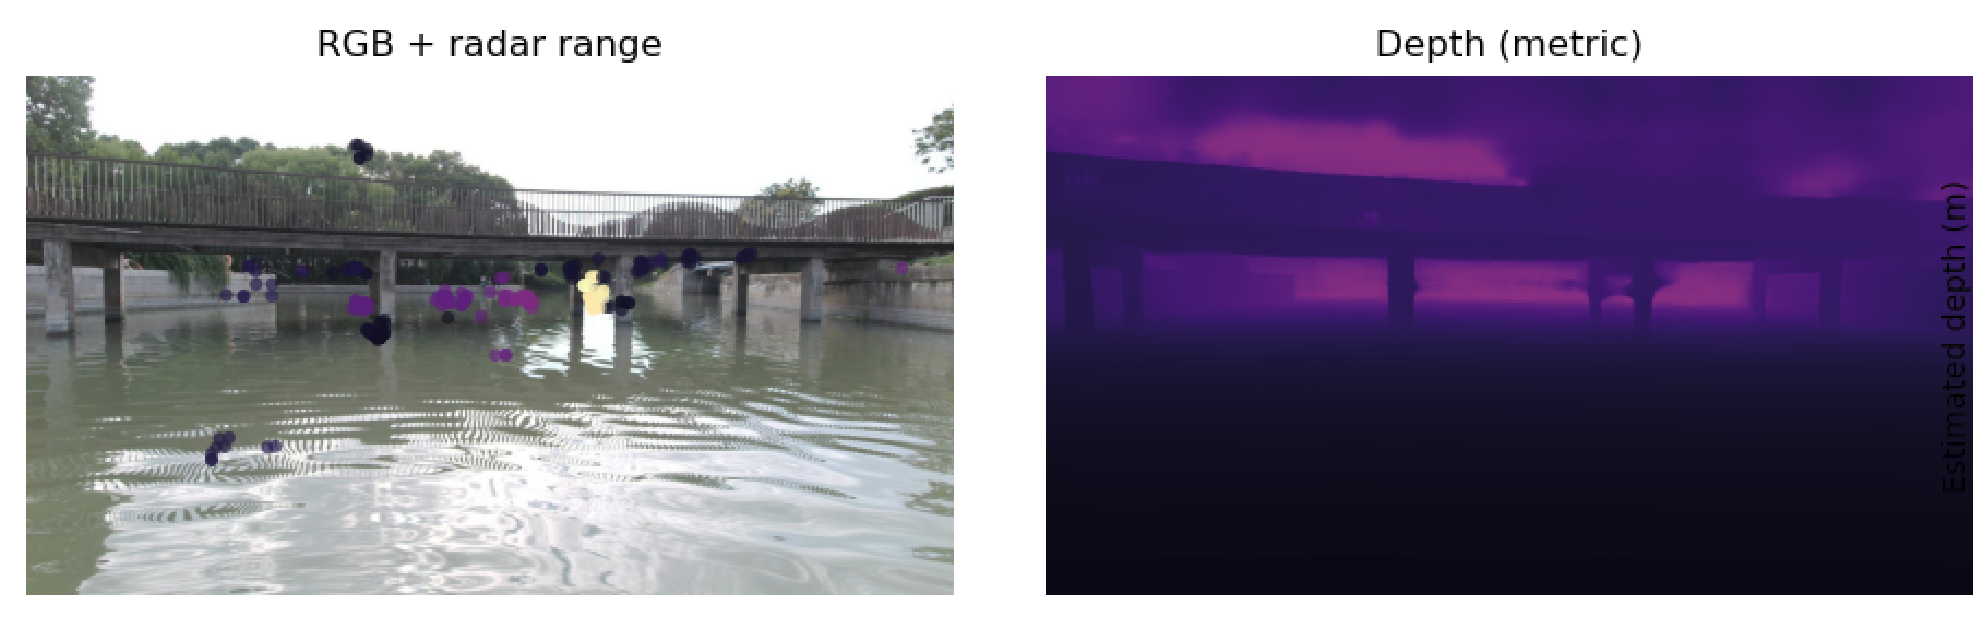
\includegraphics[width=\linewidth]{images/depth_estvsgt_1.png}\\[2pt]
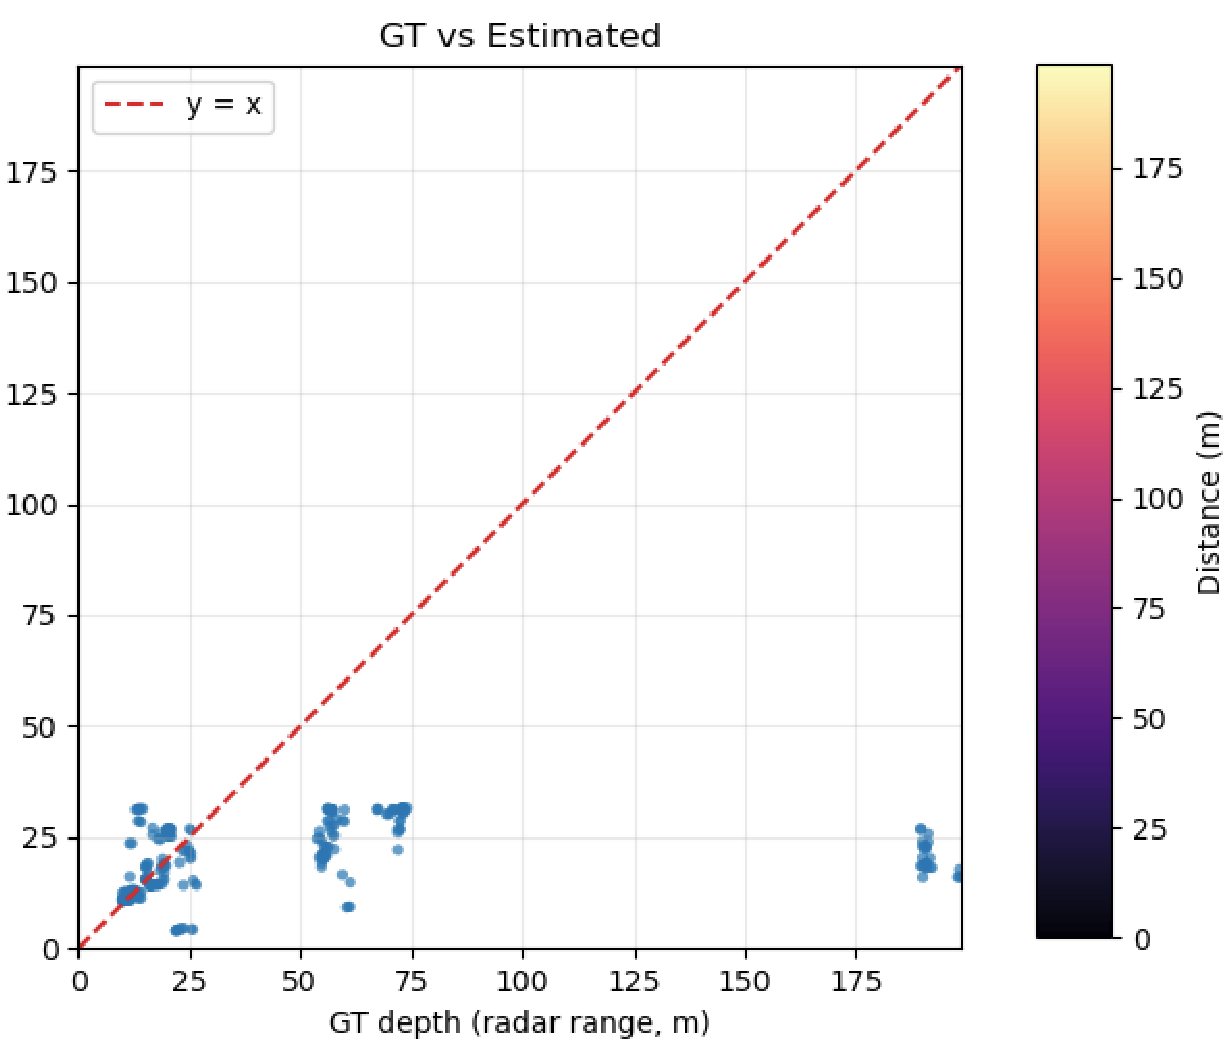
\includegraphics[width=0.8\linewidth]{images/depth_estvsgt_2.png}
\caption{Monocular depth evaluation against radar ground truth. Top: input RGB with projected radar range points (left) and the corresponding calibrated depth map (right). Bottom: estimated depth versus radar ground truth across the evaluation set; the dashed line marks perfect agreement.}
\label{fig:depth_qual}
\end{figure}

\subsection{End-to-End Pipeline Performance}
We assess end-to-end viability on real-world sequences from the MODD~\cite{Kristan2015} dataset, running the segmentation, depth, tracking, and risk-model stages together as a single pipeline. Across 419 tested frames containing tracked obstacles, the system reports 62\% SAFE, 33\% CAUTION, and 5\% IMMEDIATE, with no observed flicker between adjacent frames. The Kalman-filtered depth and velocity, the EMA-smoothed lateral offset, and the hysteresis thresholds described in Section III jointly suppress the frame-to-frame noise that would otherwise destabilize the warning signal. Figure~\ref{fig:pipeline_qual} shows two representative sequences: in the first, a tracked boat closes distance and its closing velocity rises, driving the system from SAFE through CAUTION to IMMEDIATE WARNING; in the second, a buoy produces a SAFE-to-CAUTION transition as the ASV approaches, with the overlaid track ID, distance estimate, and risk score updating consistently across frames in both cases.

\begin{figure}[t]
\centering
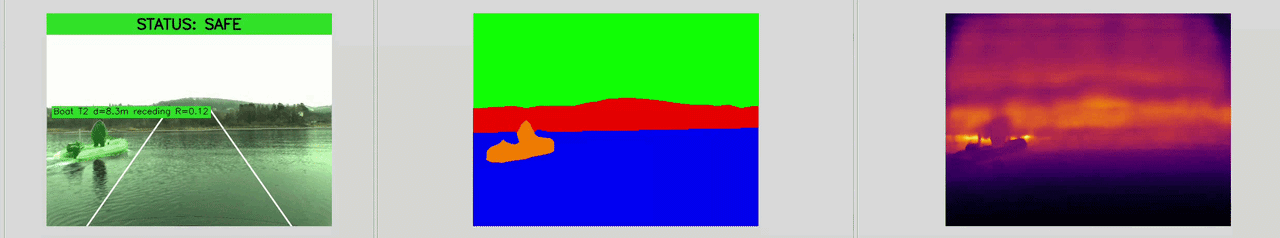
\includegraphics[width=\linewidth]{images/example1_safe.png}\\[2pt]
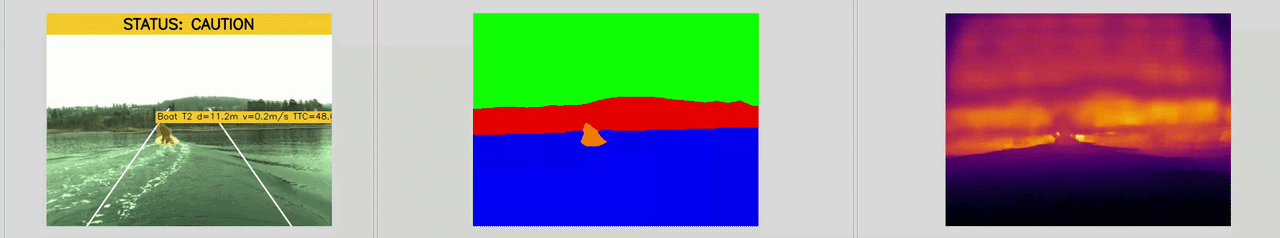
\includegraphics[width=\linewidth]{images/example1_caution.png}\\[2pt]
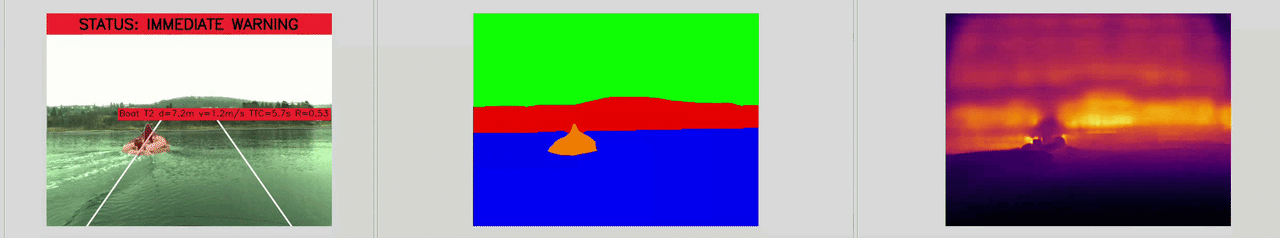
\includegraphics[width=\linewidth]{images/example1_warning.png}\\[2pt]
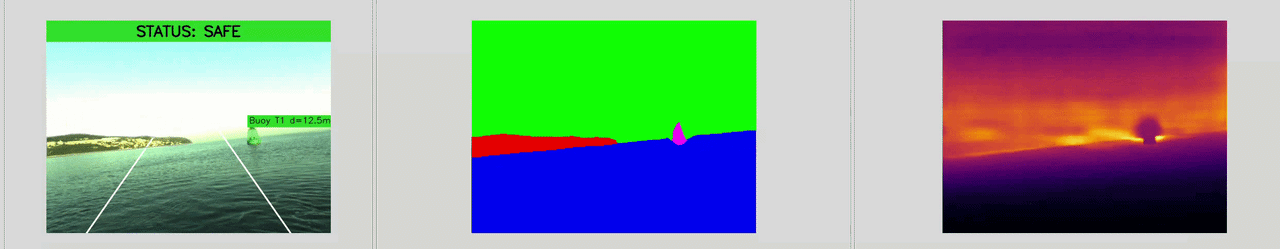
\includegraphics[width=\linewidth]{images/example2_safe.png}\\[2pt]
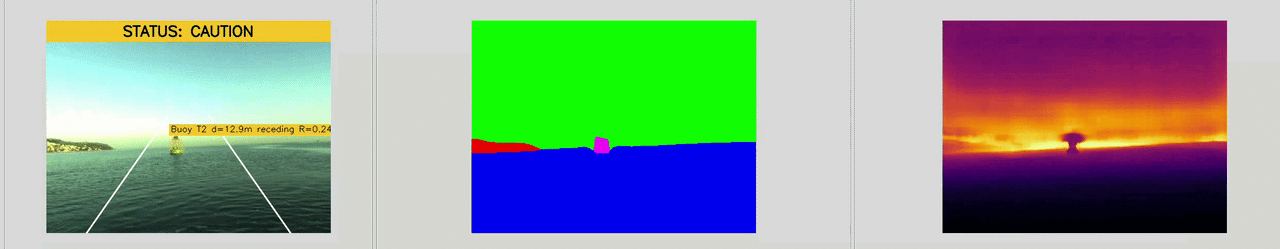
\includegraphics[width=\linewidth]{images/example2_caution.png}
\caption{Qualitative evaluation on two MODD sequences. Rows 1--3: a tracked boat closes distance and the system escalates from SAFE to CAUTION to IMMEDIATE WARNING. Rows 4--5: a tracked buoy produces a SAFE-to-CAUTION transition as the ASV approaches. Each row shows the annotated RGB frame (left), semantic segmentation (center), and monocular depth map (right).}
\label{fig:pipeline_qual}
\end{figure}

Table~\ref{tab:latency} breaks down the average per-frame latency of the full pipeline on an NVIDIA RTX 4060 GPU. Depth estimation dominates the budget at 38.7\,ms (53\% of the total), followed by segmentation at 26.9\,ms; the fusion and risk-reasoning stage adds only 7.4\,ms. The resulting total of 73.0\,ms sustains roughly 13.7\,FPS, sufficient for real-time collision warning at typical inland-vessel speeds and leaving headroom for future additions such as higher-rate sensors or more elaborate fusion logic.

\begin{table}[t]
\centering
\caption{Average inference latency of the end-to-end pipeline.}
\label{tab:latency}
\begin{tabular}{lc}
\hline
Pipeline Component & Avg.\ Latency (ms) \\
\hline
Semantic Segmentation (SegFormer) & 26.9 \\
Depth Estimation (Depth Anything V2) & 38.7 \\
Temporal Fusion \& Risk Modeling & 7.4 \\
\hline
Total System Latency & 73.0 \\
\hline
\end{tabular}
\end{table}

\subsection{Limitations}
Several limitations affect these results. Segmentation accuracy on rare hazard classes remains low (Buoy 0.2036, Swimmer 0.4254, Animal 0.0068, and Float 0.0000 IoU), so the pipeline depends on obstacle presence and coarse localization rather than fine-grained recognition. Depth calibration saturates beyond roughly 32\,m, which is acceptable for the near-field collision-warning band but leaves longer-range hazards unranged. End-to-end validation is also confined to MODD sequences from a single forward-facing camera; robustness to vessel heave and pitch, extreme lighting, and obstacles outside the camera's field of view has not yet been tested on physical hardware.

\section{Conclusion}
% We presented WARD, a lightweight, vision-only framework that bridges raw perception and actionable risk assessment. By delivering stable, human-interpretable warnings without active ranging hardware, WARD enables safe navigation for low-cost ASVs. Future work targets field deployment, 360° multi-camera coverage, and closed-loop risk-aware control.

We presented WARD, a lightweight, vision-only framework that bridges raw perception and actionable risk assessment. By fusing dual-head SegFormer segmentation with radar-calibrated Depth Anything V2 depth, WARD recovers near-range metric accuracy without the cost and complexity of active ranging hardware, while the extended SORT tracker and collision-corridor risk model turn noisy per-frame estimates into stable, human-interpretable warnings. Operating at real-time rates on a consumer-grade GPU, WARD enables safe navigation for low-cost ASVs.

Future work will pursue field deployment on a physical ASV to test robustness against vessel heave and pitch, extend the architecture to a multi-camera configuration for 360\textdegree{} situational awareness through cross-camera tracking, and close the loop by feeding the continuous risk scores into path-planning and control for autonomous evasive maneuvers. A synthetic evaluation set built with generative video models would also help offset the scarcity of annotated maritime hazard data.

% \section{Future Works}
% \input{future_works}

\section*{Acknowledgments}
AI tools such as ChatGPT and Google Gemini were used for language editing and formatting assistance.
% This work was completed as part of the final project for ROB 572 Marine Robotics at the University of Michigan, Winter 2026. 
% We acknowledge the use of AI coding assistants, such as Cursor and Google Gemini, for implementation support and writing assistance during the development of this work. The source code is available at \url{https://github.com/kevin-yiran-zhou/ROB572_project}.
% \newpage
\bibliographystyle{ieeetr}
\bibliography{references}

\end{document}